\documentclass[12]{article}

\usepackage{fullpage}
\usepackage{amsfonts}
\usepackage{amssymb}
\usepackage{amsmath}
\usepackage{graphicx}
\usepackage[margin=1in]{geometry}
\usepackage{siunitx}
\usepackage{tikz}
\usetikzlibrary{calc}

\begin{document}

\begin{flushright}
9.2, 9.3, 9.4 Write Up\\
Jim Vargas
\end{flushright}

\section{9.2 (22, 28 or 30)}
\textbf{(22): Find a vector that has the same direction as $\langle -2,4,2 \rangle$ but has length 6.}\\

To start, I will find the unit vector with the same direction as $\langle -2,4,2 \rangle$. Let $\vec{a}$ be this vector. The magnitude of $\vec{a}$ is 
\begin{eqnarray}
|\vec{a}| &=& \sqrt{{(-2)}^2 + 4^2 + 2^2}\\
&=& \sqrt{24}
\end{eqnarray}
so the unit vector with the same direction of $\vec{a}$ is $\displaystyle{
\frac{1}{\sqrt{24}} \vec{a}}$. A unit vector has a magnitude, or length, of 1, so this can be scaled to 6 by multiplying this magnitude by six. So, $\displaystyle{ \frac{6}{\sqrt{24}} \vec{a} = \Big \langle \frac{-12}{\sqrt{24}}, \frac{24}{\sqrt{24}}, \frac{12}{\sqrt{24}} \Big\rangle
}$. This vector, $\displaystyle{\Big \langle \frac{-12}{\sqrt{24}}, \frac{24}{\sqrt{24}}, \frac{12}{\sqrt{24}} \Big\rangle}$, therefore has the same direction as $\vec{a}$ and a magnitude of 6.\\

\textbf{(30): Ropes 3m and 5m in length are fastened to a holiday decoration that is suspended over a town square. The decoration has a mass of 5kg. The ropes, fastened at different heights, make angles of \ang{54} and \ang{40} with the horizontal. Find the tension in each wire and the magnitude of each tension.}
\begin{center}
\includegraphics[scale=.75]{30_FBD.png}\\
Figure 1: Free Body Diagram for Problem 30
\end{center}

Let $\mathrm{T}_1$ be the tension force on the 3m String and $\mathrm{T}_2$ be the tension force on the 5m string, indicated by Figure 1. The holiday decoration is not accelerating in any direction, so the net forces applied to the object must be zero in each direction. It follows from Newton's 2nd Law that
\begin{eqnarray}
&-mg = \mathrm{T}_1 \sin{(\ang{52})} + \mathrm{T}_2 \sin{(\ang{40})}\\
&\mathrm{T}_1 \cos{(\ang{52})} = \mathrm{T}_2 \cos{(\ang{40})}
\end{eqnarray}
By solving (4) for $\mathrm{T}_1$,
\begin{eqnarray}
\mathrm{T}_1 = \frac{\mathrm{T}_2 \cos{(\ang{40})}}{\cos{(\ang{52})}}
\end{eqnarray}
This can be substituted into (3) to solve for $\mathrm{T}_2$:
\begin{eqnarray}
-mg &=& \frac{\mathrm{T}_2 \cos{(\ang{40})}}{\cos{(\ang{52})}}\sin{(\ang{52})} + \mathrm{T}_2 \sin{(\ang{40})}\\
49\mathrm{N} &=& \mathrm{T}_2 \left( \frac{\cos{(\ang{40})}}{\cos{(\ang{52})}}\sin{(\ang{52})} + \sin{(\ang{40})} \right)\\
\frac{49\mathrm{N}}{\frac{\cos{(\ang{40})}}{\cos{(\ang{52})}}\sin{(\ang{52})} + \sin{(\ang{40})}} &=& \mathrm{T}_2\\
30.186\mathrm{N} &\approx & \mathrm{T}_2
\end{eqnarray}
It follows from (5) that $\mathrm{T}_1 \approx$ 37.559N. Finally, the tension in the 3m wire is $\mathrm{T}_1 \approx (-23.124\mathrm{N})\hat{i} + (29.597\mathrm{N})\hat{j}$ with a magnitude of 37.559N, and the tension in the 5m wire is $\mathrm{T}_2 \approx (23.124\mathrm{N})\hat{i} + (19.403\mathrm{N})\hat{j}$ with a magnitude of 30.186N.


\section{9.3 (34, 38)}
\textbf{(34): For the vectors $\vec{a} = \langle 1, 2 \rangle$ and $\vec{b} = \langle -4, 1 \rangle$, find $\mathrm{orth}_{\vec{a}} \vec{b}$ and illustrate by drawing the vectors $\vec{a},\, \vec{b},\, \mathrm{proj}_{\vec{a}} \vec{b},\, \mathrm{orth}_{\vec{a}} \vec{b}$.}\\
\begin{center}
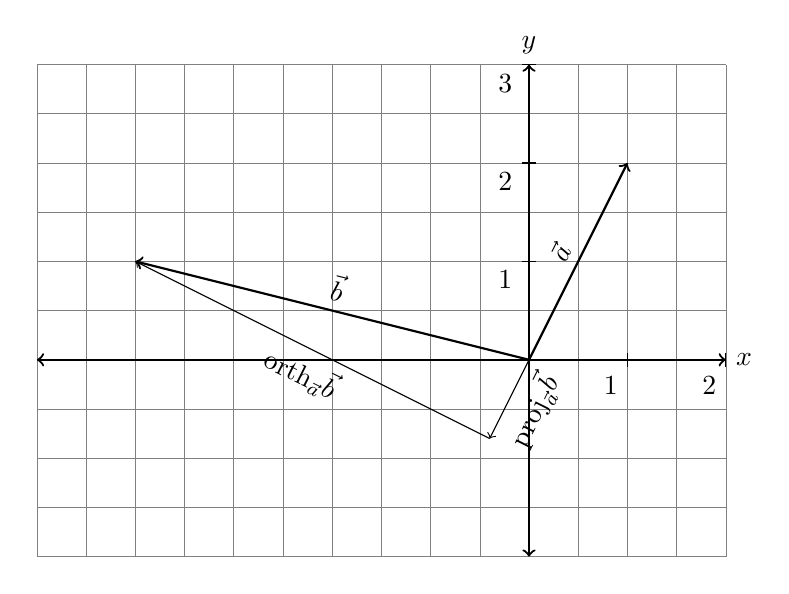
\begin{tikzpicture}[scale=1.25]
%axes
\draw[step = .5, gray, very thin] (-5, -2) grid ( 2, 3);
\draw [<->,thick] (0,3) node (yaxis) [above] {$y$}
    |- (2,0) node (xaxis) [right] {$x$};
\draw[<->, thick] (0,-2) node (yaxis) {}|- (-5,0) node (xaxis) {};
%axis labels
\foreach \x in {1,2}
   \draw (\x cm, 2pt) -- (\x cm, -2pt) node[anchor = north east] {$\x$};
\foreach \y in {1,2,3}
   \draw (2pt, \y cm) -- (-2pt, \y cm) node[anchor = north east] {$\y$};
	
%vector a
\draw[->, thick] (0,0) coordinate (a_1) -- (1,2) coordinate (a_2) node[midway,above,sloped] {$\vec a$};
%vector b
\draw[->,thick] (0,0) coordinate (b_1) -- (-4,1) coordinate (b_2) node[midway,above,sloped] {$\vec b$};
% vector proj
\draw[->] (0,0) coordinate (p_1) -- (-.4,-.8) coordinate (p_2) node[midway,below,sloped] {$\mathrm{proj}_{\vec{a}} \vec{b}$};
%vector orth
\draw[->] (p_2) -- (b_2) node[midway,below,sloped] {$\mathrm{orth}_{\vec{a}} \vec{b}$};
\end{tikzpicture}\\
Figure 2: Graph of the Vectors
\end{center}

Figure 2 shows the vectors of interest for this problem. We can see that the angle between $\vec{a}$ and $\vec{b}$ is obtuse, so $\mathrm{proj}_{\vec{a}} \vec{b}$ is negative with respect to the orientation of $\vec{a}$, and the sum of $\mathrm{proj}_{\vec{a}} \vec{b}$ and $\mathrm{orth}_{\vec{a}} \vec{b}$ will equal $\vec{b}$. Using the definition of vector projection,
\begin{eqnarray}
\mathrm{proj}_{\vec{a}} \vec{b} &=& \frac{\vec{a} \bullet \vec{b}}{{|\vec{a}|}^2}\vec{a}\\
&=& \frac{(1\cdot -4)+(2\cdot 1)}{{(1)}^2+{(2)}^2}\langle 1,2 \rangle\\
&=& \frac{-2}{5}\langle 1,2 \rangle\\
&=& \Big \langle \frac{-2}{5},\frac{-4}{5} \Big \rangle
\end{eqnarray}
Now, $\vec{b} - \mathrm{proj}_{\vec{a}} \vec{b} = \mathrm{orth}_{\vec{a}} \vec{b}$:
\begin{eqnarray}
\mathrm{orth}_{\vec{a}} \vec{b} &=& \vec{b} - \mathrm{proj}_{\vec{a}} \vec{b}\\
&=& \langle -4,1 \rangle - \Big \langle \frac{-2}{5},\frac{-4}{5} \Big \rangle\\
&=& \Big \langle (-4 - \frac{-2}{5}), (1- \frac{-4}{5}) \Big \rangle\\
&=& \Big \langle \frac{-18}{5}, \frac{9}{5} \Big \rangle
\end{eqnarray}
$\therefore$ the orthogonal projection of $\vec{b}$ onto $\displaystyle{
\vec{a}\,\, \mathrm{is}\,\, \Big \langle \frac{-18}{5}, \frac{9}{5} \Big \rangle
}$.\\

\textbf{(38): A tow truck drags a stalled car along a road. The chain makes an angle of $\ang{30}$ with the road and the tension in the chain is 1500N. How much work is done by the truck pulling the car 1km?
}\\

Work can be calculated by the scalar product of the force vector and the displacement vector:
\begin{eqnarray}
&W = \vec{F}\bullet\vec{r}\\
&W = |\vec{F}||\vec{r}|\cos{(\theta)}
\end{eqnarray}
The magnitude of the displacement vector is given as 1km, the magnitude of the tension force vector on the chain is given as 1500N, and $\theta$ is given as $\ang{30}$. Substituting these values into (19) gives
\begin{eqnarray}
W &=& (1500\mathrm{N})(1000\mathrm{m})\cos{(\ang{30})}\\
&\approx & 1299038.106\,\mathrm{N}\cdot\mathrm{m}
\end{eqnarray}
So, the truck does about $1299038\,\mathrm{N}\cdot\mathrm{m}$ of work pulling the stalled car 1km.


\section{9.4 (6, 30)}
\textbf{(6): Find the magnitude of the torque about $P$ if a 36-lb force is applied as shown.}\\
\begin{center}
\includegraphics[scale=.75]{6_FBD.png}\\
Figure 3: Diagram for Problem 6
\end{center}

The magnitude of a torque vector can be calculated by the cross product between the position vector and the force vector in the direction perpendicular to the position vector:
\begin{eqnarray}
&|\tau| = |\vec{r} \times \vec{F}|\\
&|\tau| = |\vec{r}||\vec{F}|\sin{(\theta)}
\end{eqnarray}
The magnitude of the displacement vector can be calculated as the distance between $P$ and the location where the force is applied: $|\vec{r}| = \sqrt{2({4\mathrm{ft}})^2} = 4\sqrt{2}\,\mathrm{ft}$. The magnitude of the force vector is given as a 36lb force. Figure 4 shows the free body diagram of this system, which makes the angles easier to see:
\begin{center}
\includegraphics[scale=.75]{6_FBD_2.png}\\
Figure 4: Free Body Diagram for Problem 6
\end{center}
From Figure 4, we can notice that the angle of interest is actually obtuse (dashed lines are added to show the directions perpendicular to the position vector), and is in fact $\ang{90} + (\ang{90}-\ang{30}-\ang{45})$, or $\ang{105}$. Substituting the appropriate values into (23) gives
\begin{eqnarray}
|\tau| &=& (4\sqrt{2}\,\mathrm{ft})(36\mathrm{lbs})\sin{(\ang{105})}\\
&\approx & 196.708\,\mathrm{ft\cdot lbs}
\end{eqnarray}
So, rotating the armbar contraption around $P$ with 36lbs of force will result in about $196.708\,\mathrm{ft\cdot lbs}$ of torque force about $P$.\\

\textbf{(30): Find the volume of the parallelopiped with adjacent edges $PQ$, $PR$, $PS$, given the points $P(3,0,1),\, Q(-1,2,5),\, R(5,1,-1),\, S(0,4,2)$.}\\

First, I will list the vectors:
\begin{eqnarray}
\vec{PQ} =& \langle (-1-3),(2-0),(5-1) \rangle &= \langle -4,2,4 \rangle\\
\vec{PR} =& \langle (5-3),(1-0),(-1-1) \rangle &= \langle 2,1,-2 \rangle\\
\vec{PS} =& \langle (0-3),(4-0),(2-1) \rangle &= \langle -3,4,1 \rangle
\end{eqnarray}
The volume of the parallelopiped, using the definition of a scalar triple product, is
\begin{eqnarray}
V &=& |\vec{PQ}\bullet (\vec{PR}\times\vec{PS})|\\
&=& \left| 
	\begin{vmatrix}
	-4& 2& 4\\
	2& 1& -2\\
	-3& 4& 1
	\end{vmatrix}
\right|\\
&=& \left| -4
	\begin{vmatrix}
	1& -2\\
	4& 1
	\end{vmatrix}
	-2\begin{vmatrix}
	2& -2\\
	-3& 1\\
	\end{vmatrix}
	+4\begin{vmatrix}
	2& 1\\
	-3& 4
	\end{vmatrix}
\right|\\
&=& \left|
-4[(1\cdot 1)-(-2\cdot 4)] - 2[(2\cdot 1)-(-2\cdot -3)] + 4[(2\cdot 4)-(1\cdot -3)]
\right|\\
&=& |-4(9) - 2(-4) + 4(11)|\\
&=& 16
\end{eqnarray}
$\therefore$ the volume of a parellelopiped with these dimensions is 16$u^3$.
\end{document}